\part{多元函数积分}
多元函数的积分,按照积分域的定向与否可分为无向域上的积分和有向域上的积分。无向域上的积分也称为黎曼积分,
包括定积分、二重积分、三重积分、对弧长的曲线积分和对面积的曲面积分。

\section{无向域上的积分}
在进入无向域积分的学习之前,先要了解一些基本的概念。
\begin{enumerate}
    \item \textbf{\textsf{基本域}} 是指闭区间、矩形或长方体的光滑形变,即连续可微条件下一一对应。
    \item \textbf{\textsf{简单域}} 由有限个基本域拼接而成的曲线,曲面或闭区域。
    \item \textbf{\textsf{积分域}} 指的是存在两两内部不交的(有限或无限)基本域序列$\Omega_1,\Omega_2,\cdots,\Omega_n,\cdots$,
          使得
          \[ \Omega = \Omega_1\cup\Omega_2\cup\cdots\cup\Omega_n\cup\cdots \]
          并且级数
          \[ \int_\Omega \dd\Omega = \sum_{n=1}^\infty \int_{\Omega_n} \dd\Omega \]
          收敛。
    \item \textbf{\textsf{剖分}} 基本域$\Omega_1,\Omega_2,\cdots,\Omega_n,\cdots$为$\Omega$的剖分。
          其中全体基本域的直径的最小上界称为剖分的直径。
\end{enumerate}

\begin{definition}
    设$\Omega$是积分域,$f(x)$是$\Omega$上的函数,如果对任意的$\varepsilon > 0$,都存在$\delta > 0$,
    使当$\{\Omega_n\}$为$\Omega$的直径小于$\delta$的剖分时,对每个$x_n\in\Omega_n$,都有
    \[ \abs{\sum_{n=1}^\infty f(x_n)\int_{\Omega_n} \dd\Omega - I} < \varepsilon \]
    则称实数$I$为$f(x)$在$\Omega$上的黎曼积分,记作
    \[ I = \int_\Omega f(x)\dd{\Omega} \]
\end{definition}

类似一元函数定积分,在积分域上的可积函数一定时有界函数,并且连续函数及分块连续函数都是可积函数。
\begin{theorem}
    设$f(x)$是积分域$\Omega$上有定义的函数,则$f(x)$在$\Omega$上可积$\iff$
    对于任意的$\varepsilon > 0$,都存在$\Omega$上的连续函数$\alpha(x),\beta(x)$,使得
    \begin{enumerate}[(1)]
        \item 当$x\in\Omega$,恒有$\alpha(x)\leq f(x) \leq \beta(x)$;
        \item $\displaystyle \int_\Omega [\beta(x)-\alpha(x)]\dd{\Omega} < \varepsilon$
    \end{enumerate}
\end{theorem}

\subsection{黎曼积分的性质}
定积分的线性性、区间可加性、积分单调性、积分中值性等也可以推广到多元函数的积分。
\paragraph{积分线性性}
如果$f(x),g(x)$是积分域$\Omega$上的可积函数,且$\lambda,\mu$是常数,则
\[ \int_\Omega \lambda f(x) + \mu g(x)\dd{\Omega} = \lambda\int_\Omega f(x)\dd{\Omega} + \mu\int_\Omega g(x)\dd{\Omega} \]

\paragraph{区域可加性}
如果$f(x)$是积积分域$\Omega$上的可积函数且$\Omega$可以分割成两个积分区域$\Omega_1,\Omega_2$,则
\[ \int_\Omega f(x)\dd{\Omega} = \int_{\Omega_1} f(x)\dd{\Omega} + \int_{\Omega_2} f(x)\dd{\Omega} \]

\paragraph{积分单调性}
如果$f(x),g(x)$是积分域$\Omega$上的可积函数且恒有$f(x)\leq g(x)$,则
\[ \int_\Omega f(x)\dd{\Omega} \leq \int_\Omega g(x)\dd{\Omega} \]

\paragraph{绝对单调性}
如果$f(x)$是积分域$\Omega$上的可积函数,则
\[ \abs{\int_\Omega f(x)\dd{\Omega}} \leq \int_\Omega \abs{f(x)}\dd{\Omega} \]

\paragraph{积分中值性}
如果$f(x)$是\textcolor{red}{连通}积分域$\Omega$上的\textcolor{red}{连续}函数,则存在$\xi\in\Omega$,
使得
\[ \int_\Omega f(x)\dd{\Omega} = f(\xi)\int_\Omega \dd\Omega \]

\subsection{重积分的计算}
\subsubsection{累次积分法}
对于积分域$D$上的\textcolor{red}{连续函数}$f(x,y)$,只要$D$可用不等式
\[ \alpha(x)\leq y \leq \beta(x),\quad a\leq x \leq b \]
连续表示,即$D$为$x$型区域,那么用二重积分计算公式
\begin{equation}
    \iint\limits_D f(x,y)\dd{x}\dd{y} =\int_a^b \dd{x}\int_{\alpha(x)}^{\beta(x)} f(x,y)\dd{y}
\end{equation}

如果$D$可以用不等式
\[ \varphi(y) \leq x \leq \psi(y),\quad c\leq y\leq b \]
连续表示,即$D$为$y$型区域,那么有
\begin{equation}
    \iint\limits_D f(x,y)\dd{x}\dd{y} = \int_c^b \dd{y}\int_{\varphi(y)}^{\psi(y)} f(x,y)\dd{x}
\end{equation}

如果积分区域$D$不具有上下或左右的特性,则可以对$D$适当分割,使之为上面两种区域的并接,并分别计算后求和。

对于三重积分计算,如果积分区域$\Omega$可以表示为
\[ z_\text{下}(x,y)\leq z(x,y) \leq z_\text{上}(x,y),\quad (x,y)\in D \]
则有
\begin{equation}
    \iiint\limits_\Omega f(x,y,z)\dd{x}\dd{y}\dd{z} = \iint\limits_D \dd{x}\dd{y}\int_{z_\text{下}}^{z_\text{上}}f(x,y,z)\dd{z}
\end{equation}
其中$z=z_\text{上}(x,y),z=z_\text{下}(x,y)$称为区域$\Omega$的上下边界,$D$称为区域$\Omega$的投影区域。

在围成区域$\Omega$的诸多曲面中,可以通过消去$z$的办法得到一系列不含$z$的方程,由此确定投影区域;另一方面,可以通过含有$z$的全体方程解出$z$,由此确定上下边界。
简言之,即\textbf{\textsf{找$z$解$z$定上下,缺$z$消$z$定投影}},对于$x,y$也是同理。

有时对累次积分进行积分次序交换,会简化积分的计算。
\begin{example}
    计算$\displaystyle \int_0^1\dd{x}\int_0^x\dd{y}\int_0^y\frac{\sin z}{(1-z)^2}\dd{z}$
\end{example}
\begin{solution}
    先将$x$看作为$[0,1]$的常数,交换$y,z$的积分次序,然后同法交换$x,z$的积分次序
    \begin{align*}
        I & = \int_0^1\dd{x}\int_0^x\frac{\sin z}{(1-z)^2}\dd{z}\int_z^x\dd{y} \\
          & =\int_0^1\dd{x}\int_0^x\frac{\sin z}{(1-z)^2} (x-z)\dd{z}          \\
          & = \int_0^1\frac{\sin z}{(1-z)^2}\dd{z}\int_z^1(x-z)\dd{x}          \\
          & = \int_0^1 \frac{\sin z}{(1-z)^2} \cdot \frac{1}{2}(1-z)^2\dd{z}   \\
          & = \frac{1}{2}\int_0^1\sin z\dd{z}                                  \\
          & = \frac{1}{2}(1-\cos 1)
    \end{align*}
\end{solution}

\begin{example}
    证明$\displaystyle \int_0^1\dd{x}\int_0^1 (xy)^{xy}\dd{y} = \int_0^1 x^x \dd{x}$
\end{example}
\begin{proof}
    令$t=xy$,则有$\dd{y} = \frac{1}{x}\dd{t}$,原积分可变为
    \begin{align*}
        \int_0^1\dd{x}\int_0^1 (xy)^{xy}\dd{y}
         & = \int_0^1\dd{x}\int_0^x t^t\frac{1}{x}\dd{t}  \\
         & = \int_0^1 \frac{1}{x}\dd{x}\int_0^x t^t\dd{t} \\
         & = \int_0^1 t^t\dd{t}\int_t^1 \frac{1}{x}\dd{x} \\
         & =\int_0^1 -\ln{t}\cdot t^t\dd{t}
    \end{align*}
    则只需要证明$\displaystyle\int_0^1 -\ln{x}\cdot x^x\dd{x} = \int_0^1 x^x\dd{x}$,即
    验证$\displaystyle\int_0^1 x^x(1-\ln{x})\dd{x} = 0$,事实上
    \[ \int_0^1 x^x(1-\ln{x})\dd{x} = \int_0^1 \dd{x^x} = \eval{x^x}_0^1 = 0 \]
\end{proof}

\subsubsection{利用对称性、奇偶性、轮换性计算}
设$D$是关于$y$轴对称的有界区域,且$D_1$为$D$在$y$轴右侧部分。那么有
\begin{equation}
    \iint\limits_D f(x,y) =
    \begin{cases}
        2\iint\limits_{D_1} f(x,y)\dd{x}\dd{y} & f(-x,y)=f(x,y)  \\
        0                                      & f(-x,y)=-f(x,y) \\
    \end{cases}
\end{equation}
对于积分区域关于$x$轴对称,且$f(x,y)$关于$y$具有奇偶性的情况同理。

设$D_1,D_2$是关于原点对称的有界区域,且$f(x,y)$在$D_1\cup D_2$上的连续向量函数,如果
\begin{enumerate}[(1)]
    \item $f(-x,-y)=f(x,y)$,则有$\displaystyle\iint\limits_{D_1\cup D_2}f(x,y)\dd{\sigma}=2\iint\limits_{D_1}f(x,y)\dd{\sigma}$;
    \item $f(-x,-y)=-f(x,y)$,则有$\displaystyle\iint\limits_{D_1\cup D_2}f(x,y)\dd{\sigma}=0$
\end{enumerate}

如果积分区域$D$是关于$y=x$对称,则可以将被积函数中的$x,y$相互交换。若关于$y=-x$,则可将$x,-y$相互交换。

\begin{example}
    记平面区域$D=\{ (x,y)\,|\, \abs{x}+\abs{y}\leq 1 \}$,计算如下二重积分:
    \begin{enumerate}[(1)]
        \item $\displaystyle I_1 = \iint\limits_D \frac{af(x)+bf(y)}{f(x)+f(y)}\dd{\sigma}$,其中$f(t)$为定义在$(-\infty,+\infty)$上的连续正值函数,常数$a>0,b>0$
        \item $\displaystyle I_2 = \iint\limits_D (\mathrm{e}^{\lambda x} - \mathrm{e}^{-\lambda y})$,常数$\lambda > 0$
    \end{enumerate}
\end{example}
\begin{solution}
    \begin{enumerate}[(1)]
        \item 由于$D$关于$x=y$对称,所以有
              \begin{align*}
                  I_1 & = \frac{1}{2}\iint\limits_D \frac{af(x)+bf(y)}{f(x)+f(y)} + \frac{af(y)+bf(x)}{f(y)+f(x)} \dd{\sigma} \\
                      & =\frac{(a+b)}{2}\iint\limits_D\dd{\sigma}                                                             \\
                      & =a+b
              \end{align*}
        \item 由于$D$关于$x=-y$对称,所以有
              \begin{align*}
                  I_2 & = \frac{1}{2} \iint\limits_D (\mathrm{e}^{\lambda x} - \mathrm{e}^{-\lambda y}) + (\mathrm{e}^{-\lambda y} - \mathrm{e}^{\lambda x}) \dd{\sigma} \\
                      & =0
              \end{align*}
    \end{enumerate}
\end{solution}

\begin{example}
    设$p(x)$在$[a,b]$上非负连续,$f(x)$与$g(x)$在$[a,b]$上连续且具有相同的单调性,其中$D=\{ (x,y)\,|\, a\leq x \leq b, a\leq y \leq b \}$,比较
    \[ I_1 = \iint\limits_D p(x)f(x)p(y)g(y) \dd{x}\dd{y} \text{ 与~} I_2 = \iint\limits_D p(x)f(y)p(y)g(y)\dd{x}\dd{y} \]
\end{example}
\begin{solution}
    \[ I_1 - I_2 = \iint\limits_D p(x)p(y)[f(x)g(y) - f(y)g(y)]\dd{x}\dd{y} \]
    由于$D$关于$y=x$对称,所以有
    \[ I_1 - I_2 = \iint\limits_D p(x)p(y)[f(y)g(x) - f(x)g(x)]\dd{x}\dd{y} \]
    相加得
    \begin{align*}
        I_1 - I_2 & = \frac{1}{2}\iint\limits_D p(x)p(y)[f(x)g(y) - f(y)g(y) + f(y)g(x) - f(x)g(x)]\dd{x}\dd{y} \\
                  & = \frac{1}{2}\iint\limits_D p(x)p(y)[(f(x)-f(y))g(y) + (f(y)-f(x))g(x)]\dd{x}\dd{y}         \\
                  & = \frac{1}{2}\iint\limits_D p(x)p(y)[f(x)-f(y)][g(y)-g(x)]\dd{x}\dd{y}
    \end{align*}
    由于$f(x)$与$g(x)$在$[a,b]$上具有相同的单调性,所以
    \[ [f(x)-f(y)][g(y)-g(x)] \leq 0 \]
    由$p(x),p(y)$在$[a,b]$上非负连续,所以
    \[ p(x)p(y)[f(x)-f(y)][g(y)-g(x)] \leq 0 \]
    因此有$I_1 - I_2 \leq 0$,即$I_1\leq I_2$
\end{solution}

\subsubsection{换元积分法}
在许多情况下,直接使用累次积分法计算会有很大困难,此时常用换元积分法。选择好的变量代换,对简化计算有很大的帮助。
下面介绍二元、三元的变量代换。

对于平面区域$D$,面积向量$\dd{x}\wedge \dd{y}$,若有变量代换
\[
    T:
    \begin{cases}
        x=x(u,v), \\
        y=y(u,v).
    \end{cases}
\]
则在$D_{uv}$下,面积向量$\dd{u}\wedge\dd{v}$与代换前的$\dd{x}\wedge\dd{y}$关系如下
\begin{align*}
    \dd{x} \wedge \dd{y}
     & = \left(\pdv{x}{u}\dd{u} + \pdv{x}{v}\dd{v}\right) \wedge \left(\pdv{y}{u}\dd{u} +\pdv{y}{v}\dd{v}\right) \\
     & = \pdv{x}{u}\pdv{y}{v}\dd{u}\wedge\dd{v} + \pdv{x}{v}\pdv{y}{u}\dd{v}\wedge\dd{u}                         \\
     & = \left(\pdv{x}{u}\pdv{y}{v} - \pdv{x}{v}\pdv{y}{u}\right)\dd{u}\wedge\dd{v}                              \\
     & = \pdv{(x,y)}{(u,v)}\dd{u}\wedge\dd{v}
\end{align*}
其中算符$\wedge$为外积符号,满足反交换性(三维向量的外积为叉积),于是有
\[ \dd{x}\dd{y} = \abs{\pdv{(x,y)}{(u,v)}}\dd{u}\dd{v} \]
所以二重积分的换元公式为
\begin{equation}
    \iint\limits_D f(x,y)\dd{x}\dd{y} = \iint\limits_{D_{uv}}f(x(u,v),y(u,v)) \abs{\pdv{(x,y)}{(u,v)}}\dd{u}\dd{v}
\end{equation}

同理可得三重积分的换元公式
\begin{equation}
    \iiint\limits_\Omega f(x,y,z)\dd{x}\dd{y}\dd{z} = \iiint\limits_{\Omega_{uvw}} f(x(u,v,w),\cdots)\abs{\pdv{(x,y,z)}{(u,v,w)}}\dd{u}\dd{v}\dd{w}
\end{equation}

在使用换元法时,选定好变量变换后,对区域边界进行变换,然后计算雅可比,
若雅可比中的偏导数不好求解时,可根据反函数定理,求雅可比的倒数,即换元后的变量对还原前的变量求偏导,
之后再利用换元公式计算重积分。



\subsection{常用坐标变换}
\subsubsection{极坐标变换}
对于极坐标变换
\[ x = r\cos\theta, y = r\sin\theta, (r \geq 0) \]
其雅可比为
\[
    \pdv{(x,y)}{(r,\theta)} =
    \begin{vmatrix}
        \pdv{x}{r}      & \pdv{y}{r}      \\
        \pdv{x}{\theta} & \pdv{y}{\theta}
    \end{vmatrix}
    =
    \begin{vmatrix}
        \cos\theta   & \sin\theta  \\
        -r\sin\theta & r\cos\theta
    \end{vmatrix}
    =
    r
\]
所以极坐标换元公式为
\begin{equation}
    \iint\limits_D f(x,y)\dd{x}\dd{y} = \iint\limits_{D_{r\theta}} f(r\cos\theta, r\sin\theta) r\dd{r}\dd{\theta}
\end{equation}

对于其区域的变换有如下总结
\begin{enumerate}[(i)]
    \item 如果极点在积分区域$D_{r\theta}$的外部,则常见的情况时积分区域可用不等式
          \[ \theta_1 \leq \theta \leq \theta_2, \quad r_1(\theta) \leq r(\theta) \leq r_2(\theta) \]
    \item 如果极点在积分区域$D_{r\theta}$的边界,则常见的情况是积分区域可以用不等式
          \[ \theta_1 \leq \theta \leq \theta_2,\quad 0 \leq r \leq r(\theta) \]
    \item 如果极点在积分区域$D_{r\theta}$的内部,则常见的情况是积分区域可用不等式
          \[ 0\leq 2\theta \leq 2\pi,\quad 0\leq r\leq r(\theta) \]
\end{enumerate}

\begin{situation}
    极坐标变换常用于出现$x^2+y^2$的积分(积分域)。
\end{situation}

\subsubsection{柱坐标变换}
对于柱坐标变换
\[ x=r\cos\theta, y=r\sin\theta, z=z \]
则雅可比为
\[ \pdv{(x,y,z)}{(r,\theta,z)} = r \]
此时柱坐标换元公式为
\begin{equation}
    \iiint_{\Omega} f(x,y,z)\dd{x}\dd{y}\dd{z} = \iiint_{V}f(r\cos\theta,r\sin\theta,z)r\dd{r}\dd{\theta}\dd{z}
\end{equation}

\begin{situation}
    柱坐标变换一般用于“盖子”形式的区域,即$V$可以用不等式
    \[ (r,\theta)\in D, z_1(r,\theta) \leq z \leq z_2(r,\theta) \]
    表示。
\end{situation}

\subsubsection{球坐标变换}
设$M(x,y,z)$是$xyz$空间中的一点,它在$xy$平面上的投影点为$P(x,y)$又,设$OM=r(0\leq r < \infty),OP$与$x$轴正向的夹角为$\varphi(0\leq \varphi\leq 2\pi)$,
$OM$与$z$轴正向的夹角为$\theta(0\leq\theta\leq\pi)$,则称$(r,\theta,\varphi)$为$M$点的球坐标。

即如下变换
\[
    \begin{cases}
        x = r\cos\varphi\sin\theta, \\
        y = r\sin\varphi\sin\theta, \\
        z = r\cos\theta
    \end{cases}
\]
其雅可比为
\[
    \pdv{(x,y,z)}{(r,\theta,\varphi)} =
    \begin{vmatrix}
        \cos\varphi\sin\theta & r\cos\varphi\cos\theta & -r\sin\varphi\sin\theta \\
        \sin\varphi\sin\theta & r\sin\varphi\cos\theta & r\cos\varphi\sin\theta  \\
        \cos\theta            & -r\sin\theta           & 0
    \end{vmatrix}
    = r^2\sin\theta
\]
则有球坐标变换公式
\begin{equation}
    \iiint\limits_{\Omega} f(x,y,z)\dd{x}\dd{y}\dd{z} = \iiint\limits_{V}f(r\cos\varphi\sin\theta,\cdots)r^2\sin\theta\dd{r}\dd{\theta}\dd{\varphi}
\end{equation}

\begin{situation}
    求坐标变换一般用于函数或积分域出现$x^2 + y^2 + z^2$的积分。或则积分域与球有关。
\end{situation}

\subsection{线面积分的计算}
无向曲线和无向曲面上的积分都可以通过参数化方法华为定积分或二重积分。有一些常见的曲面还可以通过单向投影或分片投影的方法实现参数化。
\subsubsection{线积分的参数化方法}
无向曲线上的积分
\[ \int_L f(x,y,z)\dd{s} \]
可以通过选择曲线$L$的参数方程来计算,如果$L$的参数方程为
\[ x=x(t), y=y(t), z=z(t) \quad (a\leq t \leq b) \]
那么根据微弧长公式
\[ \dd{s} = \sqrt{{x'_t}^2 + {y'_t}^2 + {z'_t}^2} \dd{t} \]
便可得到积分的计算公式
\begin{equation}
    \int_L f(x,y,z)\dd{s} = \int_a^b f(x(t),y(t),z(t))\sqrt{{x'_t}^2 + {y'_t}^2 + {z'_t}^2}\dd{t}
\end{equation}

特别地,当$L: x=x(t),y=y(t)$为平面曲线时,有
\begin{equation}
    \int_L f(x,y)\dd{s} = \int_a^b f(x(t),y(t)) \sqrt{{x'_t}^2 +{y'_t}^2} \dd{t}
\end{equation}

如果曲线$L:y=y(x)$可以写成参数形式$L: x=x ,y=y(x)$,所以有
\begin{equation}
    \int_L f(x,y)\dd{s} = \int_a^b f(x,y(x))\sqrt{1 + {y'_x}^2}\dd{x}
\end{equation}

如果有极坐标曲线$L: r=r(\theta)$,则有参数方程
\[ x=r(\theta)\cos\theta, y=r(\theta)\sin\theta \]
所以,有
\begin{equation}
    \int_L f(x,y)\dd{s} = \int_a^b f(r(\theta)\cos\theta,r(\theta)\sin\theta)\sqrt{r^2 + {r'_\theta}^2}\dd{\theta}
\end{equation}

利用曲线积分还可以计算一些柱面地面积。如果$S$是连接平面光滑曲线
\[ L : x=x(t),y=y(t)\quad (a\leq t\leq b) \]
与空间光滑曲线
\[ C : z=f(x,y), (x,y)\in L \]
的柱面,则当$f(x,y)\geq 0$时,$S$的面积为
\[ \int_L f(x,y)\dd{x} = \int_a^b f(x(t),y(t))\sqrt{{x'_t}^2+{y'_t}^2}\dd{t} \]

\subsubsection{面积分的参数化方法}
对于空间曲面$S$,假设它的参数方程为
\[ x=x(u,v),y=y(u,v),z=z(u,v),\quad ((u,v)\in D) \]
其向量形式为$\bm{r}=\bm{r}(u,v)$。那么其面积微元的面积向量为
\[
    \dd{\bm{S}} = \dd{\bm{r}'_u} \cross \dd{\bm{r}'_v} =
    \begin{vmatrix}
        \bm{i} & \bm{j} & \bm{k} \\
        x'_u   & y'_u   & z'_u   \\
        x'_v   & y'_v   & z'_v
    \end{vmatrix}
    \dd{u}\dd{v}
    =(A,B,C)\dd{u}\dd{v}
\]
其中
\[
    A = \pdv{(y,z)}{(u,v)},\quad B=\pdv{(z,x)}{(u,v)},\quad C=\pdv{(x,y)}{(u,v)}
\]
因此有微面积的数量公式
\begin{equation}
    \dd{S} = \sqrt{A^2+B^2+C^2}\dd{u}\dd{v}
\end{equation}
由此可得曲面面积的参数化计算公式
\begin{equation}
    \iint\limits_S f(x,y,z)\dd{S} = \iint\limits_D f(x(u,v),y(u,v),z(u,v))\sqrt{A^2+B^2+C^2}\dd{u}\dd{v}
\end{equation}

\begin{example}
    设$\Gamma : x=x(t),y=y(t)\,(a\leq t \leq b)$为一平面参数曲线,试求$\Gamma$绕$x$轴得到的旋转曲面的面积。
\end{example}
\begin{solution}
    设旋转曲面为$S$,则$S$的参数化形式为
    \[ x = x(t), y = y(t)\cos\theta, z=y(t)\sin\theta,\quad (a\leq t \leq b, 0\leq \theta \leq 2\pi) \]
    则有
    \begin{align*}
        A & = \pdv{(y,z)}{(t,\theta)} =
        \begin{vmatrix}
            y'(t)\cos\theta & -y(t)\sin\theta \\
            y'(t)\sin\theta & y(t)\cos\theta
        \end{vmatrix}
        =y'(t)y(t)                      \\
        B & = \pdv{(z,x)}{t,\theta} =
        \begin{vmatrix}
            y'(t)\sin\theta & y(t)\cos\theta \\
            x'(t)           & 0
        \end{vmatrix}
        =x'(t)y(t)\cos\theta            \\
        C & = \pdv{(x,y)}{(t,\theta)} =
        \begin{vmatrix}
            x'(t)           & 0               \\
            y'(t)\cos\theta & -y(t)\sin\theta
        \end{vmatrix}
        = -x'(t)y(t)\sin\theta
    \end{align*}
    因此有
    \[
        \iint\limits_S \dd{S}
        =
        \iint\limits_D \sqrt{A^2+B^2+C^2}\dd{t}\dd{\theta}
        =
        2\pi\int_a^b y(t)\sqrt{{x'_t}^2+{y'_t}^2}\dd{t}
    \]
\end{solution}

对于参数曲面$\bm{r} = \bm{r}(u,v)$
根据勾股定理
\[ \sqrt{A^2+B^2+C^2} = \norm{\bm{r}'_u\cross\bm{r}'_v} = \sqrt{{\bm{r}'_u}^2 + {\bm{r}'_v}^2 - (\bm{r}'_u\bm{r}'_v)^2} \]
所以微面积公式可以写成
\[ \dd{S} = \sqrt{{\bm{r}'_u}^2 + {\bm{r}'_v}^2 - (\bm{r}'_u\bm{r}'_v)^2} \dd{u}\dd{v} \]
相应的曲面积分的计算公式可以写成
\begin{equation}
    \iiint\limits_S f(x,y,z)\dd{S} = \iint\limits_D f(x(u,v),y(u,v),z(u,v))\sqrt{EG-F^2}\dd{u}\dd{v}
\end{equation}
其中$E = {\bm{r}'u}^2, F=\bm{r}'_u\bm{r}'_v, G={\bm{r}'_v}^2$

求解$E,F,G$可以用下面的方法
\begin{equation}
    \dd{\bm{r}^2} = \dd{x^2} + \dd{y^2} + \dd{z^2} =E\dd{u^2}+2F\dd{u}\dd{v}+G\dd{v^2}
\end{equation}

\begin{example}
    求曲面$(x^2+y^2+z^2)^2 = a^2(x^2+y^2-z^2)$的面积
\end{example}
\begin{solution}
    曲面的参数方程如下
    \[ x=r\cos\varphi\sin\theta, y=r\sin\varphi\sin\theta,z=r\cos\theta \]
    曲面方程变为
    \[ r = a\sqrt{-\cos 2\theta},\quad (\frac{1}{4}\pi \leq \theta \leq \frac{3}{4}\pi) \]
    计算微分
    \begin{align*}
          & \dd{x^2} + \dd{y^2} + \dd{z^2}                                                                                               \\
        = & [\dd(r\cos\varphi\sin\theta)]^2 + [\dd(r\sin\varphi\sin\theta)]^2 + [\dd(r\cos\theta)]^2                                     \\
        = & [\cos\varphi\dd(r\sin\theta) - r\sin\theta\sin\varphi \dd{\varphi}]^2                                                        \\
          & +[\sin\varphi\dd(r\sin\theta) +r\sin\theta\cos\varphi\dd{\varphi}]^2                                                         \\
          & +[\dd(r\cos\theta)]^2                                                                                                        \\
        = & [\dd{(r\sin\theta)}]^2 + r^2\sin^2\theta\dd{\varphi^2} + [\dd{(r\cos\theta)}]^2                                              \\
        = & [\sin\theta\dd{r} + r\cos\theta\dd{\theta}]^2 + r^2\sin^2\theta\dd{\varphi^2} + [\cos\theta\dd{r} -r\sin\theta\dd{\theta}]^2 \\
        = & \dd{r^2} + r^2\dd{\theta^2} + r^2\sin^2\theta\dd{\varphi^2}                                                                  \\
        = & ({r'_\theta}^2 + r^2)\dd{\theta^2} + r^2\sin^2\theta\dd{\varphi^2}                                                           \\
    \end{align*}
    所以,有
    \[ EG-F^2 = ({r'_\theta}^2 + r^2)r^2\sin^2\theta \]
    则所求面积微
    \begin{align*}
        S & = \iint\limits_S \dd{S} = \iint\limits_D \sqrt{EG-F^2}\dd{\theta}\dd{\varphi}               \\
          & = \iint\limits_S \sqrt{r^2 + {r'_\theta}^2} r\sin\theta\dd{\theta}\dd{\varphi}              \\
          & = \int_0^{2\pi}\dd{\varphi}\int_{\frac{1}{4}\pi}^{\frac{3}{4}\pi} a^2 \sin\theta\dd{\theta} \\
          & = 2\sqrt{2}\pi a^2
    \end{align*}
\end{solution}

\subsubsection{曲面积分的投影方法}
如果曲面$S: z=z(x,y)\,(x,y)\in D$的参数方程为
\[ x=x, y=y, z=z(x,y) \]
所以有$(A,B,C)=(-z'_x,-z'_y,1)$,由此可得
\begin{equation}
    \iint\limits_S f(x,y,z)\dd{S} = \iint\limits_D f(x,y,z(x,y))\sqrt{{z'_x}^2 + {z'_y}^2 + 1}\dd{x}\dd{y}
\end{equation}
其中$D$为曲面$S$在$xOy$平面上的投影。投影方法的特点是:找$z$解$z$定偏导,缺$z$消$z$定投影。

投影方法其实为面积投影公式的另一种表述,即微面积有如下关系
\[ \dd{x}\dd{y} = \cos\gamma\dd{S} \]
其中$\gamma$为$xOy$平面与微曲面$\dd{S}$的夹角,也就是向量$(0,0,1)$与$(-z'_x, -z'_y, 1)$的夹角。
因而有
\[ \cos\gamma = \frac{1}{\sqrt{{z'_x}^2 + {z'_y}^2 + 1}} \]

\begin{example}
    设有一高度为$h(t)$的雪堆在融化,其中$t$为时间,其侧面方程为$z=h(t)-\dfrac{2(x^2+y^2)}{h(t)}$,已知体积减少的速率与侧面积成正比(比例系数为$0.9$),
    问高度为$130$的雪堆全部融化需要多少时间。(长度单位为厘米,时间单位为小时)
\end{example}
\begin{solution}
    设所需时间为$T$,根据题意可以得出下列关系式
    \begin{align*}
        D         & : x^2+y^2\leq \frac{1}{2}h^2(t)                             \\
        \dv{V}{t} & = -0.9S                                                     \\
        S         & = \iint\limits_D \sqrt{{z'_x}^2 + {z'_y}^2 + 1}\dd{x}\dd{y} \\
        V         & = \iint\limits_D \dd{x}\dd{y}\int_0^{z(x,y,t)} \dd{z}       \\
    \end{align*}
    先计算体积$V$,
    \begin{align*}
        V & = \iint\limits_D \dd{x}\dd{y}\int_0^{z(x,y,t)} \dd{z}                                                 \\
          & = \iiint\limits_D h(t)-\frac{2(x^2+y^2)}{h(t)}\dd{x}\dd{y}                                            \\
          & = \int_0^{2\pi} \dd{\theta}\int_0^{\frac{1}{\sqrt{2}}h(t)} \left(h(t)-\frac{2r^2}{h(t)}\right)r\dd{r} \\
          & = \frac{\pi}{4}h^3(t)
    \end{align*}
    接着计算侧面积$S$,
    \begin{align*}
        S & = \iint\limits_D \sqrt{{z'_x}^2 + {z'_y}^2 + 1}\dd{x}\dd{y}                                               \\
          & = \iint\limits_D \sqrt{\frac{16}{h^2(t)}(x^2+y^2) + 1} \dd{x}\dd{y}                                       \\
          & = \int_0^{2\pi} \dd{\theta} \int_0^{\frac{1}{\sqrt{2}}h(t)} \sqrt{\frac{16}{h^2(t)}r^2 + 1} \vdot r\dd{r} \\
          & = \frac{13}{12}\pi h^2(t)
    \end{align*}
    因此有
    \[ \dv{V}{t} = \frac{3}{4}\pi h^2(t) h'(t) = -\frac{9}{10} \frac{13}{12}\pi h^2(t) \]
    得$h'(t) = -\dfrac{13}{10}$,因此$h(t)=-\dfrac{13}{10}t + C$,根据$h(0)=130$可得$C=130$
    所以由$h(T)=0$解得$T=100$。所以高度$130$厘米的雪堆全部融化需要$100$小时。
\end{solution}

\subsection{黎曼积分的应用}
\subsubsection{重心的计算}
按照黎曼积分的定义,分布在积分域$\Omega$上的连续介质,其质量密度为$\rho(x,y,z)$时,总质量为
\[ m = \int_\Omega f(x,y,z)\dd{\Omega} \]

对于给定质点系$(\bm{r}_i,m_i)\,(i=1,2,3,\cdots)$,物理上称指点位置关于质量的加权平均为\textcolor{red}{\textbf{\textsf{重心}}}。
即
\[ \overline{\bm{r}} = \sum_{i=1}^{n} \frac{m_i}{m}\bm{r}_i, \quad m = \sum_{i=j}^n m_j \]
积分形式为
\begin{equation}
    \overline{\bm{r}} = \frac{1}{m}\int_\Omega \bm{r} \rho(\bm{r})\dd{\Omega}
\end{equation}

其中$\rho(\bm{r})\dd{\Omega}$对应$m_i$,$\bm{r}$对应$\bm{r}_i$。
分量形式为
\begin{align}
    \overline{x} = \frac{1}{m}\int_\Omega x\rho(x,y,z)\dd{\Omega} \\
    \overline{y} = \frac{1}{m}\int_\Omega y\rho(x,y,z)\dd{\Omega} \\
    \overline{z} = \frac{1}{m}\int_\Omega z\rho(x,y,z)\dd{\Omega}
\end{align}
其中$\displaystyle m = \int_\Omega \rho(x,y,z)\dd{\Omega}$

\section{有向域上的积分}
定向域上的积分简称为定向类积分。
\subsection{定向类曲线积分}
定向曲线上的积分习惯称为\textcolor{red}{\textbf{\textsf{第二型曲线积分}}},场见问题由变力作功和向量场环量等。

指定了参数表示类型的曲线称为\textcolor{red}{\textbf{\textsf{定向曲线}}}。一个曲线只有正反两种情况,但定向的表示可以时多种多样的。
例如光滑曲线可以指定切向类来表示定向;曲线弧段可以通过指定首尾端点表示定向;封闭曲线可以通过指定相对的左旋右旋来表示定向;参数曲线可以指定
参数的增减来表示定向等等。

\begin{definition}
    设$L:x=x(t),y=y(t),z=z(t)\,(a\leq t\leq b)$是基本曲线且按照参数增长定向,又设$P,Q,R$是$L$上的可积函数,
    如果有
    \[ \int_L P\dd{x} + Q\dd{y} + R\dd{z} = \int_a^b (Px'(t) + Qy'(t) + Rz'(t))\dd{t} \]
    则称实数
    \[ \int_L P\dd{x} + Q\dd{y} + R\dd{z} \]
    为定向类曲线积分。
\end{definition}
定向类曲线积分可以这么理解
\[ \int_L P\dd{x} + Q\dd{y} + R\dd{z} = \int_L (P,Q,R) \vdot (\dd{x},\dd{y},\dd{z}) = \int_L \bm{f}(\bm{r}) \vdot \dd{\bm{r}} \]
即在曲线$L$上的微元$\dd{\bm{r}}$与此点处的向量函数$\bm{f}(\bm{r})$的点乘,进行全曲线上的累积。
所以定向类曲线积分可以看作是向量函数在定向曲线上\textcolor{red}{投影}的积分。

\begin{theorem}
    设$L$为定向的基本曲线,且$\bm{f}$是$L$上的连续向量函数,如果$L$有两种不同的参数化光滑地表示$\bm{r} = \bm{r}_1(t)\,(a\leq t\leq b),\, \bm{r}=\bm{r}_2(s)\, (c\leq s \leq d)$
    则有
    \[ \int_a^b \bm{f}\vdot\bm{r}_1'(t)\dd{t} = \int_c^d \bm{f}\vdot\bm{r}_2'(s)\dd{s} \]
\end{theorem}

\begin{theorem}
    设$L$是定向的基本曲线,若$(\cos\alpha,\cos\beta,\cos\gamma)$是$(x,y,z)\in L$的指定切向量,则有
    \[ \int_L P\dd{x} + Q\dd{y} + R\dd{z} = \int_L (P\cos\alpha + Q\cos\beta + R\cos\gamma)\dd{s} \]
    其中$\bm{r} =\bm{r}(s)\,(0\leq s\leq b),\, \dd{\bm{r}} = (\cos\alpha,\cos\beta,\cos\gamma)\dd{s}$
    且$s$为弧长。
\end{theorem}

\begin{theorem}
    设$L^+, L^-$是同一曲线积分域的两个相反定向表示,若$\bm{f}$是该曲线上的可积向量函数,则有
    \[ \int_{L^+} \bm{f}\vdot\dd{\bm{r}} = - \int_{L^-}\bm{f}\vdot\dd{\bm{r}} \]
\end{theorem}

\subsubsection{曲线积分的计算}
计算定向类曲线积分,最基本的方法就是参数化方法或分段参数化方法。
\begin{enumerate}[(1)]
    \item 构造并写出曲线的参数方程;
    \item 利用参数方程吧曲线积分化为定积分,即带入参数方程并按照曲线的定向确定定积分的上下限,当参数按照参数递增方向定向时,下限取参数的最小值,上限去参数的最大值;
    \item 计算定积分即可得出结果。
\end{enumerate}

\subsection{有向曲面上的积分}
定向类曲面积分又称\textcolor{red}{\textbf{\textsf{第二型曲面积分}}}
\subsubsection{定向类曲面积分}
考虑一个流速函数$\bm{v}$,其流体通过某个微平面$\dd{\bm{S}}$,所以在单位时间内通过这个微平面的数量为
\[ \bm{v}\vdot\dd{\bm{S}} = \bm{v}\vdot(\bm{r}'_u \cross \bm{r}'_v)\dd{u}\dd{v} = (\bm{v},\bm{r}'_u,\bm{r}'_v)\dd{u}\dd{v} \]
由此流体穿过曲面$S$的总数量为
\[ \iint\limits_S \bm{v}\vdot\dd{\bm{S}} = \iint\limits_D (\bm{v},\bm{r}'_u,\bm{r}'_v)\dd{u}\dd{v} \]

根据外积运算
\[ (\dd{y}\wedge\dd{z}, \dd{z}\wedge\dd{x}, \dd{x}\wedge\dd{y}) = \left(\pdv{(y,z)}{(u,v)},\pdv{(z,x)}{(u,v)},\pdv{(x,y)}{(u,v)}\right)\dd{u}\wedge\dd{v} \]
由于曲面$S$按照$\bm{r}'_u\cross\bm{r}'_v$定向,所以有
\begin{align*}
    \dd{\bm{S}}
     & = (\bm{r}'_u\cross\bm{r}'_v)\dd{u}\dd{v}                                                  \\
     & = (\bm{r}'_u\cross\bm{r}'_v)\dd{u}\wedge\dd{v}                                            \\
     & = \left(\pdv{(y,z)}{(u,v)},\pdv{(z,x)}{(u,v)},\pdv{(x,y)}{(u,v)}\right)\dd{u}\wedge\dd{v} \\
     & = (\dd{y}\wedge\dd{z}, \dd{z}\wedge\dd{x}, \dd{x}\wedge\dd{y})                            \\
     & = (\dd{y}\dd{z},\dd{z}\dd{x},\dd{x}\dd{y})
\end{align*}

此外也可以根据面积投影公式\ref{eq:面积投影公式}可知
\[ \dd{\bm{S}} = (\cos\alpha,\cos\beta,\cos\gamma)\dd{S} = (\cos\alpha\dd{S},\cos\beta\dd{S},\cos\gamma\dd{S}) = (\dd{y}\dd{z},\dd{z}\dd{x},\dd{x}\dd{y}) \]

综上可以将定向类曲面积分定义为
\begin{definition}
    设$S:\bm{r}=\bm{r}(u,v),((u,v)\in D)$是基本曲面且按照$\bm{r}'_u\cross\bm{r}'_v$定向,
    又设$P,Q,R$是$S$上的可积函数,如果有
    \[ \iint\limits_S P\dd{y}\dd{z} + Q\dd{z}\dd{x} + R\dd{x}\dd{y} = \iint\limits_D (\bm{v},\bm{r}'_u,\bm{r}'_v)\dd{u}\dd{v} \]
    其中$\bm{v}=(P,Q,R)$,则称
    \[ \iint\limits_S P\dd{y}\dd{z} + Q\dd{z}\dd{x} + R\dd{x}\dd{y} \]
    为定向类曲面积分。
\end{definition}

与定向类曲线积分一样,定向类曲面积分也有如下定理
\begin{theorem}
    设$S$是定向的基本曲面,且$\bm{v}$是$S$上的连续向量函数,如果$\bm{r}=\bm{r}_1(u,v)\,(u,v)\in D_1$和$\bm{r}=\bm{r}_2(s,t)\,(s,t)\in D_2$
    都是$S$的同向光滑表示,则有
    \[ \iint\limits_{D_1} (\bm{v},\bm{r}'_u, \bm{r}'_v)\dd{u}\dd{v} = \iint\limits_{D_2} (\bm{v},\bm{r}'_s,\bm{r}'_t)\dd{s}\dd{t} \]
\end{theorem}

\begin{theorem}
    设$S$为定向的基本曲面,且$(P,Q,R)$是$S$上的连续向量函数。如果$(\cos\alpha,\cos\beta,\cos\gamma)$是$(x,y,z)\in S$上的指定法向量,则有
    \[ \iint\limits_S P\dd{y}\dd{z} + Q\dd{z}\dd{x} + R\dd{x}\dd{y} = \iint\limits_S (P\cos\alpha + Q\cos\beta + R\cos\gamma) \dd{S} \]
\end{theorem}

\subsubsection{曲面积分的计算}
定向类曲面积分的基本算法有参数化方法,单向投影法和分片投影法。
\paragraph{参数化方法}
对于定向曲面$S$,如果其参数方程$\bm{r}=\bm{r}(u,v)\,(u,v)\in D$,即
\[ x=x(u,v),y=y(u,v),z=z(u,v) \]
\textcolor{red}{同时需要满足$\bm{r}'_u,\bm{r}'_v,\bm{n}$为右手系},其中$\bm{n}$为曲面$S$的指定方向。
则有
\begin{align*}
    \iint\limits_S P\dd{y}\dd{z} + Q\dd{z}\dd{x} + R\dd{x}\dd{y}
     & = \iint\limits_D (\bm{v},\bm{r}'_u, \bm{r}'_v) \dd{u}\dd{v} \\
     & = \iint\limits_D (PA+QB+RC)\dd{u}\dd{v}                     \\
     & = \iint\limits_D
    \begin{vmatrix}
        P    & Q    & R    \\
        x'_u & y'_u & z'_u \\
        x'_v & y'_v & z'_v
    \end{vmatrix}
    \dd{u}\dd{v}
\end{align*}

\paragraph{单向投影法}
如果曲面积分域可以用显式方程
\[ z=f(x,y),\quad (x,y)\in D \]
表示,即$\bm{r} = \bm{r}(x,y,f(x,y))$,则可以用上下侧表示定向。当$S$为上侧时,则有法向量为
\[ \bm{r}'_x\cross\bm{r}'_y = (-z'_x, -z'_y, 1) \]
所以曲面积分的上侧投影公式为
\begin{equation}
    \iint\limits_S P\dd{y}\dd{z} + Q\dd{z}\dd{x} + R\dd{x}\dd{y} = \iint\limits_D (P,Q,R)\vdot(-z'_x,-z'_y,1)\dd{x}\dd{y}
\end{equation}
其中$D$为曲面$S$在平面$xOy$的投影区域。

对于下侧的投影公式为
\begin{equation}
    \iint\limits_S P\dd{y}\dd{z} + Q\dd{z}\dd{x} + R\dd{x}\dd{y} = \iint\limits_D (P,Q,R)\vdot(z'_x,z'_y,-1)\dd{x}\dd{y}
\end{equation}

在计算积分的时候,对于单向投影法来说,常常需要把积分域分为上下两个曲面,然后分别计算定向曲面积分,最后再相加起来。

\paragraph{分片投影法}
当曲面积分域不能用一个显式方程表示时,可以将积分域分片,向不同的坐标面进行投影。
\begin{example}
    计算曲面积分
    \[ I = \iint\limits_\Sigma \frac{x\dd{y}\dd{z} + z^2\dd{x}\dd{y}}{x^2+y^2+z^2} \]
    其中$\Sigma$时由曲面$x^2+y^2=R^2$及两平面$z=R,z=-R\,(R>0)$所围成立体表面的外侧。
\end{example}
\begin{solution}
    令
    \begin{align*}
        P & = \frac{x}{x^2 + y^2 + z^2}   \\
        Q & = 0                           \\
        R & = \frac{z^2}{x^2 + y^2 + z^2}
    \end{align*}
    将$\Sigma$分为上、侧、下,三个面,则有
    \[ I = \iint\limits_{\Sigma_1} + \iint\limits_{\Sigma_2} + \iint\limits_{\Sigma_3} = I_1 + I_2 + I_3 \]
    其中$\Sigma_1,\Sigma_3$在$xOy$平面的投影区域均为$D : x^2+y^2\leq R^2$,则有
    \[ I_1 = \iint_D (P,Q,R)\vdot(0,0,1)\dd{x}\dd{y} = \iint\limits_D R\dd{x}\dd{y} \]
    \[ I_3 = \iint_D (P,Q,R)\vdot(0,0,-1)\dd{x}\dd{y} = -\iint\limits_D R\dd{x}\dd{y} \]
    所以有$I_1+I_3=0$

    对$\Sigma_2$,进行参数化,设$x=R\cos\theta, y=R\sin\theta, z=z$
    则有$\bm{r}'_\theta,\bm{r}'_z,\bm{n}$构成右手系,其中$\bm{n}$为侧面的给定方向。
    \begin{align*}
        A & = \pdv{(y,z)}{(\theta,z)} = R\cos\theta \\
        B & = \pdv{(z,x)}{(\theta,z)} = R\sin\theta \\
        C & = \pdv{(x,y)}{(\theta,z)} = 0
    \end{align*}
    所以
    \begin{align*}
        I_2 & = \iint\limits_{\Omega_2} (P,Q,R)\vdot(A,B,C)\dd{\theta}\dd{z}                \\
            & =\int_0^{2\pi}\dd{\theta}\int_{-R}^R \frac{R^2\cos^2\theta}{R^2 + z^2} \dd{z} \\
            & = \frac{\pi}{2}R\int_0^{2\pi} \cos^2\theta \dd{\theta}                        \\
            & =\frac{1}{2}R\pi^2
    \end{align*}
\end{solution}

\subsection{定向类积分公式}
格林公式、高斯公式、斯托克斯公式,这三个公式能将定向曲线积分、定向曲面积分、重积分进行相互转化。
\begin{theorem}
    (格林公式)
    \label{th:格林公式}
    设$D$是平面简单域,$\Gamma$为其边界。若$P(x,y),Q(x,y)$在$D$上有\textcolor{red}{连续的偏导数},则按照$\Gamma$逆时针定向,有
    \[ \int_\Gamma P(x,y)\dd{x} + Q(x,y)\dd{y} = \iint\limits_D \left(\pdv{Q}{x} - \pdv{P}{y}\right) \dd{x}\dd{y} \]
\end{theorem}
\begin{theorem}
    (高斯公式)
    \label{th:高斯公式}
    设$\Omega$是三维简单域。若$P(x,y,z),Q(x,y,z),R(x,y,z)$在$\Omega$上有\textcolor{red}{连续的偏导数},则按照边界$\Sigma$的外侧定向,有
    \begin{align*}
        \iint\limits_\Sigma P\dd{y}\dd{z} + Q\dd{z}\dd{x} + R\dd{x}\dd{y}
         & =\iiint\limits_\Omega \left(\pdv{P}{x} + \pdv{Q}{y} + \pdv{R}{z}\right) \dd{x}\dd{y}\dd{z} \\
         & =\grad\vdot{(P,Q,R)}\dd{x}\dd{y}\dd{z}
    \end{align*}
\end{theorem}
\begin{theorem}
    (斯托克斯公式)
    设$\Sigma$是定向的二维简单域且$\Gamma$为其按照右手法则定向的边界。若$P(x,y,z),Q(x,y,z),R(x,y,z)$在$\Sigma$上有\textcolor{red}{连续的偏导数},
    则有
    \[
        \int_\Gamma P\dd{x} + Q\dd{y} + R\dd{z}
        =
        \iint\limits_\Sigma
        \begin{vmatrix}
            \dd{y}\dd{z} & \dd{z}\dd{x} & \dd{x}\dd{y} \\
            \pdv{x}      & \pdv{y}      & \pdv{z}      \\
            P            & Q            & R
        \end{vmatrix}
        =\curl{(P,Q,R)}\vdot(\dd{y}\dd{z},\dd{z}\dd{x},\dd{x}\dd{y})
    \]
\end{theorem}

\subsubsection{格林公式的应用}
对于平面上的曲线积分,当偏导数差$\pdv*{Q}{x}-\pdv*{P}{y}$比较简单,特别是$0$或常数时,通常用格林公式来计算;
当积分路径不具体或比较复杂时,通常需要格林来修改积分路径

\paragraph{化二重积分为曲线积分}
在格林公式中,如果令$P=-y,Q=x$,则有
\[ 2\iint\limits_D \dd{x}\dd{y} = \int_\Gamma x\dd{y} - y\dd{x} \]
由此可得平面区域$D$的线积分面积公式
\[ \iint\limits_D \dd{x}\dd{y} = \frac{1}{2} \int_\Gamma x\dd{y}-y\dd{x} \]
此时再通过定向曲线积分的计算方法(参数化)来进行计算。

\paragraph{化曲线积分为二重积分}
当积分表达式比较复杂或积分路径不容易参数化(例如抽象曲线)的平面曲线积分,通常用格林公式来计算。如果路径不是封闭的曲线,通常需要补充一段,使其变为封闭曲线。
一般补充的曲线为直线,且最好是沿某一坐标方向的直线。

同时要注意使用格林公式时,边界所围成的区域要有连续的偏导数$\pdv{Q}{x},\pdv{P}{y}$,
对于偏导数不连续或不存在的点,常常需要在此点构造一个圆形小邻域$V$,然后在新区域$D/V$的上使用格林公式,此时有
\begin{equation}
    \int_{\partial D} = \int_{\partial D+\partial V} - \int_{\partial V} = \iint\limits_{D/V} - \int_{\partial V}
\end{equation}
其中$\partial D,\partial V$分别表示区域$D,V$的边界,$\partial D$按\textcolor{red}{逆时针定向},$\partial V$按\textcolor{red}{顺时针定向}。
这类问题可形象地称为“有洞打洞”问题。

\begin{example}
    计算曲线积分
    \[ I = \int_L\frac{-y}{x^2+y^2}\dd{x}+\frac{x}{x^2+y^2}\dd{y} \]
    其中$L$是一个不过原点,分段光滑且按逆时针定向地简单封闭曲线。
\end{example}
\begin{solution}
    这里$L$是一个抽象曲线,显然应该使用格林公式。设$L$包围地区域为$D$。令
    \[ P = \frac{-y}{x^2+y^2},\quad Q = \frac{x}{x^2+y^2} \]
    则有
    \[ \pdv{Q}{x} = \pdv{P}{y} = \frac{y^2}{(x^2+y^2)^2} \]
    那么需要对$(0,0)$点处进行分类讨论。
    \begin{enumerate}[(1)]
        \item 当$(0,0)\notin D$时,则有
              \[ I = \iint\limits_D \left(\pdv{Q}{x}-\pdv{P}{y}\right) \dd{x}\dd{y} = \iint\limits_D 0 \dd{x}\dd{y} = 0 \]
        \item 当$(0,0)\in D$时,原点为奇点,那么对于充分小地$\varepsilon > 0$,取区域$V: x^2+y^2 < \varepsilon^2$,则可在闭区域$D/V$上应用格林公式。
              \begin{align*}
                  I & = \int_{L+\partial V} - \int_{\partial V} = \iint\limits_{D/V} 0\dd{x}\dd{y} - \int_{\partial V}                                                                    \\
                    & = 0 + \int_0^{2\pi} \frac{-\varepsilon\sin\theta}{\varepsilon^2} \dd(\varepsilon\cos\theta) + \frac{\varepsilon\cos\theta}{\varepsilon^2}\dd(\varepsilon\sin\theta) \\
                    & = \int_0^{2\pi} \dd{\theta}                                                                                                                                         \\
                    & = 2\pi
              \end{align*}
    \end{enumerate}
\end{solution}

\begin{example}
    设$f(x,y)$式$\{ (x,y)\,|\, x^2+y^2\leq 1 \}$上的二阶连续可微函数,满足$\displaystyle\pdv[2]{f}{x}+\pdv[2]{f}{y}=x^2y^2$,计算积分
    \[ I = \iint\limits_{x^2+y^2\leq 1} \left(\frac{x}{\sqrt{x^2+y^2}}\pdv{f}{x} + \frac{y}{\sqrt{x^2+y^2}}\pdv{f}{y}\right)\dd{x}\dd{y} \]
\end{example}
\begin{solution}
    由于题中给出了含二阶偏导数的条件,所以关键在于如何将被积函数向二阶偏导上变形。考虑到格林公式有$\displaystyle\pdv{Q}{x}-\pdv{P}{y}$的形式,与条件上的关联。
    变形的关键在于二重积分中,先将一个变量看作常数,然后则有一个定积分,再联系线积分的参数化计算,则可以得出下面解题思路。

    利用极坐标变换有
    \begin{align*}
        I & = \int_0^{2\pi}\dd{\theta}\int_0^1 \left(\cos\theta \pdv{f}{x} + \sin\theta\pdv{f}{y}\right)r\dd{r}            \\
          & = \int_0^1 \dd{r}\int_0^{2\pi} r\cos\theta \pdv{f}{x} + r\sin\theta\pdv{f}{y}\dd{\theta}                       \\
          & = \int_0^1 \dd{r} \int_0^{2\pi} \left(-\pdv{f}{y},\pdv{f}{x}\right)\vdot(-r\sin\theta, r\cos\theta)\dd{\theta} \\
          & = \int_0^1 \dd{r} \oint\limits_{x^2+y^2 = r^2} \left(-\pdv{f}{y},\pdv{f}{x}\right)\cdot(\dd{x},\dd{y})         \\
          & = \int_0^1 \dd{r} \iint\limits_{x^2+y^2\leq r^2} \pdv[2]{f}{x} + \pdv[2]{f}{y} \dd{x}\dd{y}                    \\
          & = \int_0^1 \dd{r} \iint\limits_{x^2+y^2\leq r^2} x^2y^2 \dd{x}\dd{y}                                           \\
          & = \int_0^1 \dd{r} \int_0^{2\pi} \dd{\theta}\int_0^r t^4\sin^2\theta\cos^2\theta \cdot t \dd{t}                 \\
          & = \int_0^1 \dd{r} \int_0^{2\pi} \sin^2\theta\cos^2\theta \dd{\theta}\int_0^r t^5 \dd{t}                        \\
          & = \frac{1}{6}\int_0^1 r^6 \dd{r} \int_0^{2\pi} \sin^2\theta\cos^2\theta\dd{\theta}                             \\
          & = \frac{1}{42}\cdot 2\mathrm{B}\left(\frac{3}{2},\frac{3}{2}\right)                                            \\
          & = \frac{\pi}{168}
    \end{align*}
\end{solution}

\begin{example}
    设$f(x,y)$为具有二阶连续偏导数的二次齐次函数,即对任意$x,y,t$下式成立
    \[ f(tx,ty) = t^2f(x,y) \]
    设$D$是由$L:x^2+y^2=4$正向一周所围成的闭区域,证明
    \[ \oint_L f(x,y)\dd{s} = \iint\limits_D \laplacian f(x,y) \dd{\sigma} \]
\end{example}
\begin{proof}
    等式两边同时对$t$求导得
    \[ xf'_1(tx,ty) + yf'_2(tx,ty) = 2tf(x,y) \]
    令$t=1$得
    \[ x\pdv{f}{x} + y\pdv{f}{y} = 2f(x,y) \]
    那么有
    \begin{align*}
        \oint_L f(x,y)\dd{s}
         & = \frac{1}{2} \oint_L \left(x\pdv{f}{x} + y\pdv{f}{y}\right)\dd{s}                   \\
         & =  \oint_L \left(-\pdv{f}{y},\pdv{f}{x}\right) \vdot(-\frac{y}{2},\frac{x}{2})\dd{s} \\
         & =  \oint_L \left(-\pdv{f}{y},\pdv{f}{x}\right) \vdot\dd{\bm{s}}                      \\
         & = \iint\limits_D \laplacian f(x,y) \dd{\sigma}
    \end{align*}
\end{proof}

\begin{example}
    设$L$为曲线$x^2+y^2=R^2$一周,$\bm{n}$为$L$的外法线方向向量,$u(x,y)$具有二阶连续偏导数且$\displaystyle \pdv[2]{u}{x} + \pdv[2]{u}{y}=x^2+y^2$。
    求$\displaystyle\oint_L \pdv{u}{\bm{n}}\dd{s}$
\end{example}
\begin{solution}
    \[
        \pdv{u}{\bm{n}}
        = \grad{u}\vdot\bm{n}_0
        = \left(\pdv{u}{x},\pdv{u}{y}\right)\vdot\left(\frac{x}{R},\frac{y}{R}\right)
        = \left(-\pdv{u}{y},\pdv{u}{x}\right)\vdot\left(-\frac{y}{R},\frac{x}{R}\right)
        = \left(-\pdv{u}{y},\pdv{u}{x}\right)\vdot\bm{t}_0
    \]
    其中$\bm{n}_0$为外法线的单位方向向量,$\bm{t}_0$为曲线上逆时针方向的单位切向量。
    故原积分为
    \begin{align*}
        \oint_L \pdv{u}{\bm{n}}\dd{s}
         & = \oint_L \left(-\pdv{u}{y},\pdv{u}{x}\right)\vdot\bm{t}_0\dd{s} \\
         & = \iint\limits_{x^2+y^2\leq R^2} \laplacian{u} \dd{x}\dd{y}      \\
         & = \iint\limits_{x^2+y^2\leq R^2} x^2+y^2 \dd{x}\dd{y}            \\
         & = \int_0^{2\pi} \dd{\theta} \int_0^R r^2\cdot r \dd{r}           \\
         & =\frac{\pi}{2}R^4
    \end{align*}
\end{solution}
上面两个都有一个知识点,就是如何将无向域的线积分变为定向线积分,即如何将被积函数化成向量场与曲线单位切向量的内积。

\begin{example}
    已知平面区域$D=\{ (x,y)\,|\, x^2+y^2\leq 1 \}$,$L$为$D$的边界正向一周。证明:
    \[ I = \oint_L \frac{x\mathrm{e}^{\sin y}\dd{y} - y\mathrm{e}^{-\sin x}\dd{x}}{4x^2+5y^2} \geq \frac{2}{5}\pi \]
\end{example}
\begin{proof}
    此题关键在于提前优化被积函数的表达,以简化在格林公式中的求导步骤。

    由于在$L$上有
    \[ 4x^2+5y^2 = 4 + y^2 = 5 - x^2 \]
    所以
    \begin{align*}
        I & = \oint_L -\frac{y\mathrm{e}^{-\sin x}}{5-x^2}\dd{x} + \frac{x\mathrm{e}^{\sin y}}{4 + y^2}\dd{y}                                \\
          & = \iint\limits_D \frac{\mathrm{e}^{\sin y}}{4+y^2} + \frac{\mathrm{e}^{-\sin x}}{5-x^2} \dd{x}\dd{y}                             \\
          & = \iint\limits_D \frac{\mathrm{e}^{\sin y}}{4+y^2}\dd{x}\dd{y} + \iint\limits_D\frac{\mathrm{e}^{-\sin x}}{5-x^2} \dd{x}\dd{y}   \\
          & \geq \frac{1}{5}\left(\iint\limits_D \mathrm{e}^{\sin y} \dd{x}\dd{y} + \iint\limits_D \mathrm{e}^{-\sin x} \dd{x}\dd{y} \right) \\
          & = \frac{1}{5}\left(\iint\limits_D \mathrm{e}^{\sin x} \dd{x}\dd{y} + \iint\limits_D \mathrm{e}^{-\sin x} \dd{x}\dd{y} \right)    \\
          & = \frac{1}{5}\iint\limits_D \mathrm{e}^{\sin x} + \mathrm{e}^{-\sin x} \dd{x}\dd{y}                                              \\
          & \geq \frac{1}{5}\iint\limits_D 2\sqrt{\mathrm{e}^{\sin x}\cdot\mathrm{e}^{-\sin x}} \dd{x}\dd{y}                                 \\
          & = \frac{2}{5}\iint\limits_D \dd{x}\dd{y}                                                                                         \\
          & = \frac{2}{5}\pi
    \end{align*}

\end{proof}


\subsubsection{高斯公式的应用}
对于定向类曲面积分,如果封闭曲面由多个光滑曲面构成,用参数化方法或投影方法可能会成倍地增加计算量。遇到这种情况,一般可用高斯公式将曲面积分转化为三重积分来计算。
\begin{example}
    计算曲面积分
    \[ I =\iint_{\Sigma} x^3\dd{y}\dd{z} + y^3\dd{z}\dd{x} + z^3\dd{x}\dd{y} \]
    其中$\Sigma$是球面$x^2+y^2+z^2=R^2$的外侧。
\end{example}
\begin{solution}
    \begin{enumerate}[(1)]
        \item 用高斯公式。曲面$\Sigma$的包围闭区域为$\Omega$,则有
              \begin{align*}
                  I & = \iiint\limits_{\Omega} \left(\pdv{P}{x} + \pdv{Q}{y} + \pdv{R}{z}\right)\dd{x}\dd{y}\dd{z}                     \\
                    & =\iiint\limits_{\Omega} 3(x^2+y^2+z^2)\dd{x}\dd{y}\dd{z}                                                         \\
                    & =3\int_0^{2\pi}\dd{\varphi}\int_0^{\pi}\dd{\theta}\int_0^{R} r^2\vdot r^2\sin\theta \dd{r} = \frac{12}{5}\pi R^5
              \end{align*}
        \item 单向投影法。根据对称性,有
              \begin{align*}
                  I & = 3\iint\limits_\Sigma z^3\dd{x}\dd{y} =3\left(\iint\limits_{\Sigma_\text{上}}+\iint\limits_{\Sigma_\text{下}}\right)z^3\dd{x}\dd{y} \\
                    & = 3\iint\limits_{x^2+y^2\leq R^2} (0,0,z_\text{上}^3)\vdot(-z'_{\text{上}x},-z'_{\text{上}y},1)
                  + (0,0,z_\text{下}^3)\vdot(z'_{\text{下}x},z'_{\text{下}y},-1)\dd{x}\dd{y}                                                               \\
                    & = 6\iint\limits_{x^2+y^2\leq R^2} (\sqrt{R^2 - x^2 - y^2})^3 \dd{x}\dd{y}                                                            \\
                    & = 6\int_0^{2\pi}\dd{\varphi}\int_0^R \left(\sqrt{R^2 - r^2}\right)^3 r\dd{r} = \frac{12}{5}\pi R^5
              \end{align*}
        \item 参数化算法。根据球面方程
              \[ x=R\cos\varphi\sin\theta, y=R\sin\varphi\sin\theta, z=R\cos\theta \]
              \[ (0\leq \varphi \leq 2\pi, 0\leq \theta \leq \pi) \]
              则$\bm{r}'_\theta, \bm{r}'_\varphi, \bm{n}$构成右手系,其中$\bm{n}$为球面法向量。
              \begin{align*}
                  A & = \pdv{(y,z)}{(\theta,\varphi)} = R^2\cos\varphi\sin^2\theta \\
                  B & = \pdv{(z,x)}{(\theta,\varphi)} = R^2\sin\varphi\sin^2\theta \\
                  C & = \pdv{(x,y)}{(\theta,\varphi)} = R^2\sin\theta\cos\theta
              \end{align*}
              因此有
              \begin{align*}
                  I & =  \iint\limits_\Sigma (x^3,y^3,z^3)\vdot(A,B,C)\dd{\theta}\dd{\varphi}                                                                    \\
                    & =     \iint\limits_\Sigma (R^5\cos^4\varphi\sin^5\theta + R^5\sin^4\varphi\sin^5\theta + R^5\cos^4\theta\sin\theta)\dd{\theta}\dd{\varphi} \\
                    & =     R^5\int_0^{2\pi}\dd{\varphi}\int_0^{\pi} (\cos^4\varphi + \sin^4\varphi)\sin^5\theta + \cos^4\theta\sin\theta\dd{\theta}             \\
                    & =     R^5\left(\int_0^{2\pi} \cos^4\varphi \dd{\varphi}\int_0^{\pi}\sin^5\theta\dd{\theta}
                  + \int_0^{2\pi} \sin^4\varphi \dd{\varphi}\int_0^{\pi}\sin^5\theta\dd{\theta}\right.                                                           \\
                    & + \left.\int_0^{2\pi} \dd{\varphi}\int_0^{\pi} \cos^4\theta\sin\theta\dd{\theta}\right)                                                    \\
                    & = R^5\left(2B\left(\frac{1}{2},\frac{5}{2}\right)B\left(3,\frac{1}{2}\right)
                  + 2B\left(\frac{5}{2},\frac{1}{2}\right)B\left(3,\frac{1}{2}\right)
                  +2\pi B\left(1,\frac{5}{2}\right)\right)                                                                                                       \\
                    & =R^5\left(4B\left(\frac{1}{2},\frac{5}{2}\right)B\left(3,\frac{1}{2}\right)+2\pi B\left(1,\frac{5}{2}\right)\right)                        \\
                    & =\frac{12}{5}\pi R^5
              \end{align*}
    \end{enumerate}
\end{solution}

这三种解法相比,显然是高斯公式更加简便,特别当$\grad\vdot{(P,Q,R)} = \left(\pdv{P}{x}+\pdv{Q}{y}+\pdv{R}{z}\right)$比较简单时,比如$0$或常数,高斯公式具有明显优势。
在解题中,应根据实际情况选择不同的方法。

对于非封闭曲面也可以用高斯公式,这类问题常常可以通过添加一些简单的曲面(特别时平面)使其封闭。这类问题可以形象地称为“缺盖补盖”问题。
此时高斯公式可以描述为
\[ \iint\limits_\Sigma = \iint\limits_{\Sigma+\Sigma_1} - \iint\limits_{\Sigma_1} = \iiint\limits_\Omega - \iint\limits_{\Sigma_1} \]

\subsubsection{斯托克斯公式地应用}
利用斯托克斯公式可以将参数化比较困难或分段太多地曲线积分转化为积分域或积分表达式相对简单地曲面积分。

\begin{example}
    计算曲线积分
    \[ I = \int_L z\dd{x} + x\dd{y} + y\dd{z} \]
    其中$L$是平面$x+y+z=1$被三个坐标面所截得三角形$S$的边界,从$x$轴正向看去,曲线$L$是逆时针方向。
\end{example}
\begin{solution}
    计算向量场$(P,Q,R)=(z,x,y)$的旋度,有
    \[ \curl{(P,Q,R)} = (1,1,1) \]
    按照斯托克斯公式,有
    \begin{align*}
        I & = \int_L z\dd{x} + x\dd{y} + y\dd{z}
        = \iint\limits_S \curl{(P,Q,R)}\vdot(\dd{y}\dd{z},\dd{z}\dd{x},\dd{x}\dd{y}) \\
          & = \iint\limits_S \dd{y}\dd{z} + \dd{z}\dd{x} + \dd{x}\dd{y}              \\
    \end{align*}
    其中$S$的定向为上侧,根据对称性有
    \[ I = 3\iint\limits_S \dd{x}\dd{y} = \frac{3}{2} \]
\end{solution}

\begin{example}
    计算曲线积分
    \[ I = \int_L (y^2-z^2)\dd{x} + (z^2-x^2)\dd{y} + (x^2-y^2)\dd{z} \]
    其中$L$是平面$x+y+z=\frac{3}{2}$截正方体$[0,1;0,1;0,1]$所得多边形的边界,从$z$轴正向看去,
    曲线$L$是逆时针方向。
\end{example}
\begin{solution}
    计算向量场$(P,Q,R)=(y^2-z^2, z^2-x^2, x^2-y^2)$的旋度
    \[ \curl{(P,Q,R)} = -2(y+z, z+x, x+y) \]
    根据斯托克斯公式,有
    \begin{align*}
        I & = \int_L P\dd{x} + Q\dd{y} + R\dd{z}                                         \\
          & = \iint\limits_S \curl{(P,Q,R)}\vdot(\dd{y}\dd{z},\dd{z}\dd{x},\dd{x}\dd{y}) \\
          & = -2\iint\limits_S (y+z)\dd{y}\dd{z} + (z+x)\dd{z}\dd{x} + (x+y)\dd{x}\dd{y}
    \end{align*}
    其中$S$为上侧定向,设$S$在$xOy$平面上的投影区域为$D$。则$D$可以表示为
    \[ D: D_1 \cup D_2 \]
    \[ D_1 : 0\leq x\leq \frac{1}{2},\quad \frac{1}{2} - x \leq y \leq 1  \]
    \[ D_2 : \frac{1}{2}\leq x\leq 1,\quad 0 \leq y \leq \frac{3}{2} - x  \]
    由于显式方程$z=\dfrac{3}{2}-x-y$可得面积向量$(1,1,1)$,此时根据单向投影法有
    \begin{align*}
        I & = -2\iint\limits_S (y+z)\dd{y}\dd{z} + (z+x)\dd{z}\dd{x} + (x+y)\dd{x}\dd{y} \\
          & =-2\iint\limits_D (y+z,z+x,x+y)\vdot(1,1,1)\dd{x}\dd{y}                      \\
          & =-2\iint\limits_D 2(x+y+z)\dd{x}\dd{y}                                       \\
          & =-6\iint\limits_D\dd{x}\dd{y}
    \end{align*}
    根据投影域的几何关系可得投影域面积为正方形区域减去两个等边直角三角形区域。
    \begin{figure}[H]
        \centering
        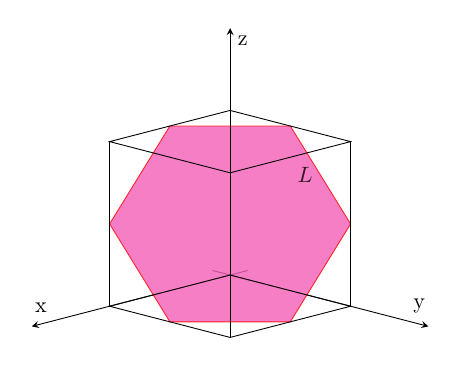
\begin{tikzpicture}[scale=0.8]
            \begin{axis}[
                    view={135}{15},
                    axis lines=center,
                    axis equal,
                    xmin=0, ymin=0, zmin=0, xmax=1.5, ymax=1.5, zmax=1.5,
                    xlabel=x,
                    ylabel=y,
                    zlabel=z,
                    ticks=none
                ]
                \draw[color=red,opacity=0.8,fill=CarnationPink] (axis cs:0,0.5,1) -- (axis cs:0.5,0,1) -- (axis cs: 1,0,0.5)
                -- (axis cs:1,0.5,0) -- (axis cs:0.5,1,0) -- (axis cs:0,1,0.5) -- cycle node [color=black,left,pos=0.5] {$L$};
                \draw (axis cs:0,0,0) -- (axis cs:1,0,0) -- (axis cs:1,1,0) -- (axis cs:0,1,0) --cycle;
                \draw (axis cs:0,0,1) -- (axis cs:1,0,1) -- (axis cs:1,1,1) -- (axis cs:0,1,1) --cycle;
                \draw (axis cs:0,0,0) -- (axis cs:0,0,1);
                \draw (axis cs:1,0,0) -- (axis cs:1,0,1);
                \draw (axis cs:0,1,0) -- (axis cs:0,1,1);
                \draw (axis cs:1,1,0) -- (axis cs:1,1,1);
            \end{axis}
        \end{tikzpicture}
        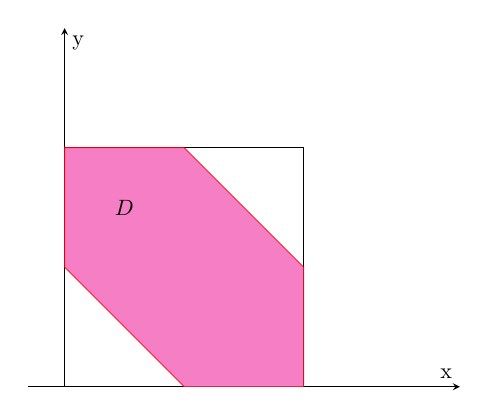
\begin{tikzpicture}[scale=0.8]
            \begin{axis}[
                    axis lines=center,
                    axis equal,
                    xmin=0, ymin=0, xmax=1.5, ymax=1.5,
                    xlabel=x,
                    ylabel=y,
                    ticks=none
                ]
                \draw (axis cs:0,0) -- (axis cs:1,0) -- (axis cs:1,1) -- (axis cs:0,1) -- cycle;
                \draw[color=red,opacity=0.8,fill=CarnationPink] (axis cs:0.5,0) -- (axis cs:1,0)
                -- (axis cs:1,0.5) -- (axis cs:0.5,1) -- (axis cs:0,1) -- (axis cs:0,0.5) -- cycle;
                \node at (axis cs:0.25,0.75) {$D$};
            \end{axis}
        \end{tikzpicture}
    \end{figure}
    \[ S_D = 1 - 2\times\frac{1}{2}\times\frac{1}{2}\times\frac{1}{2} = \frac{3}{4} \]
    故有
    \[ I = -6 S_D= -\frac{9}{2} \]
\end{solution}

\begin{example}
    计算$\displaystyle I=\oint_L (y^2-z^2)\dd{x} + (2z^2-x^2)\dd{y} + (3x^2-y^2)\dd{z}$,其中$L$是平面$x+y+z=2$与柱面$\abs{x}+\abs{y}=1$的交线,
    从$z$轴正向往负向看$L$,$L$为逆时针方向。
\end{example}
\begin{solution}
    向量场$(P,Q,R)=(y^2-z^2, 2z^2-x^2, 3x^2-y^2)$,则有
    \[ \curl(P,Q,R) = (-2y-4z, -2z-6x, -2x-2y) = -2(y+2z, z+3x, x+y) \]
    则有
    \[
        I = \oint_L P\dd{x} + Q\dd{y} R\dd{z}= -2\iint\limits_S (y+2z, z+3x, x+y)\vdot \dd{\bm{S}}
    \]
    其中$S$为$L$所的平面区域,方向为平面$x+y+z=2$的法向量方向。故有
    \begin{align*}
        I & = -2\iint\limits_S (y+2z, z+3x, x+y)\vdot(\frac{1}{\sqrt{3}},\frac{1}{\sqrt{3}},\frac{1}{\sqrt{3}})\dd{S} \\
          & =-\frac{2}{\sqrt{3}} \iint\limits_S 4x+2y+3z \dd{S}                                                       \\
          & =-\frac{2}{\sqrt{3}} \iint\limits_S x - y +6 \dd{S}                                                       \\
          & =-\frac{2}{\sqrt{3}} \iint\limits_D (x - y +6)\sqrt{1+(-1)^2+(-1)^2} \dd{x}\dd{y}                         \\
          & = -2 \iint\limits_D (x - y +6) \dd{x}\dd{y}                                                               \\
    \end{align*}
    其中$D$为$S$在平面$xOy$的投影区域,即$\abs{x}+\abs{y}=1, z=0$,根据$D$对称性,与$x,y$的奇偶性可知
    \[ I = -2 \iint\limits_D 6 \dd{x}\dd{y} = -12 \iint\limits_D \dd{x}\dd{y} = -24 \]
\end{solution}

\begin{example}
    设$\Sigma$为球面$x^2+y^2+z^2=1$的外侧,计算
    \[ I = \oiint\limits_\Sigma \frac{2}{x\cos^2 x}\dd{y}\dd{z} + \frac{1}{\cos^2 y}\dd{z}\dd{x} - \frac{1}{z\cos^2 z}\dd{x}\dd{y} \]
\end{example}
\begin{solution}
    对于复杂的积分,首先要考虑的是化简。对于此题来说,比较麻烦的是分子是三角函数。所以要利用对称性和奇偶性来化简。
    \begin{align*}
        I & = \oiint\limits_\Sigma \frac{2}{x\cos^2 x}\dd{y}\dd{z} + \frac{1}{\cos^2 y}\dd{z}\dd{x} - \frac{1}{z\cos^2 z}\dd{x}\dd{y}                                        \\
          & = \oiint\limits_\Sigma \left(\frac{2}{x\cos^2 x} , \frac{1}{\cos^2 y} , -\frac{1}{z\cos^2 z}\right)\vdot(x,y,z)\dd{\sigma}                                       \\
          & = \oiint\limits_\Sigma \frac{2}{\cos^2 x} + \frac{y}{\cos^2 y} - \frac{1}{\cos^2 z} \dd{\sigma}                                                                  \\
          & = 2\oiint\limits_\Sigma \frac{}{\cos^2 x} \dd{\sigma} + \oiint\limits_\Sigma \frac{y}{\cos^2 y} \dd{\sigma} -\oiint\limits_\Sigma \frac{1}{\cos^2 z} \dd{\sigma} \\
          & = 2I_1 + I_2 - I_3
    \end{align*}
    根区间对称性可知$I_1 = I_3$,根据函数奇偶性和区间对称性可知$I_2=0$,故
    \begin{align*}
        I & = \oiint\limits_\Sigma \frac{1}{\cos^2 z} \dd{\sigma}                                                      \\
          & = 2\iint\limits_{x^2+y^2\leq 1} \frac{1}{\cos^2 z}\frac{1}{z}\dd{x}\dd{y}                                  \\
          & = 2\int_0^{2\pi} \dd{\theta} \int_0^1 \frac{1}{\cos[2](\sqrt{1-r^2})} \frac{1}{\sqrt{1-r^2}}\cdot r \dd{r} \\
          & = -2\int_0^{2\pi} \dd{\theta}\int_0^1 \frac{1}{\cos[2](\sqrt{1-r^2})} \dd{\sqrt{1-r^2}}                    \\
          & = -2\int_0^{2\pi} \dd{\theta}\int_0^1  \dd{\tan(\sqrt{1-r^2})}                                             \\
          & = 4\pi\tan 1
    \end{align*}
\end{solution}

\subsection{场的微分与积分}
按照方向性,场可以分为数量场和向量场;按照时间相关性,场可以分为稳定场和非稳定场。

在有关场的问题中,经常会出现一个运算$\grad$,称为Hamilton算子,读作Nabla,表示对空间中某点作梯度运算。
\[ \grad = \left(\pdv{x},\pdv{y},\pdv{z}\right) \]
对于一个向量场$\bm{f}=(P(x,y,z),Q(x,y,z),R(x,y,z))$,其散度和旋度分别为
\[ \grad\vdot{\bm{f}} = \pdv{P}{x} + \pdv{Q}{y} + \pdv{R}{z} \]
\[
    \curl{\bm{f}} =
    \begin{vmatrix}
        \bm{i}  & \bm{j}  & \bm{k}  \\
        \pdv{x} & \pdv{y} & \pdv{z} \\
        P       & Q       & R
    \end{vmatrix}
\]

对于两个Hamilton算子的点积称为Laplace算子,记作
\[ \laplacian = \grad \vdot \grad = \pdv[2]{x} + \pdv[2]{y} + \pdv[2]{z} \]

\subsubsection{数量场与梯度场}
数量场的变化规律可以用梯度场表示,由数量场的梯度构成的向量场称为\textbf{\textsf{梯度场}}。

\paragraph{梯度的运算法则}
由于梯度运算是一种求导法则,那么根据求导公式不难得出梯度的运算法则
\begin{enumerate}[(1)]
    \item (线性性)$\grad(\lambda u + \mu v) = \lambda\grad{u} + \mu\grad{v}$;
    \item (乘积公式)$\grad(uv) = v\grad{u} + u\grad{v}$;
    \item (除法公式)$\grad(\dfrac{u}{v}) = \dfrac{v\grad{u}-u\grad{v}}{v^2}$;
    \item (复合公式)$\grad{F(u)} = F'(u)\grad{u}$;
    \item (复合公式)$\grad{F(u,v)} = \pdv{F}{u}\grad{u} + \pdv{F}{v}\grad{v}$
\end{enumerate}
其中$u,v$是数量场,$\lambda,\mu$是常数。

梯度场的积分域积分域的单连通性\sn{直观地说,单连通空间中所有闭曲线都能连续地收缩至一点}相关。
其相关性可以由如下定理给出
\begin{theorem}
    设$\Omega$是单连通的区域,若$P(x,y,z),Q(x,y,z),R(x,y,z)$是$D$内的偏导连续函数,则下列五个条件等价:
    \begin{enumerate}[(1)]
        \item (环量恒零性)当$L$是$\Omega$内的分段光滑的简单封闭曲线时,恒有
              \[ \int_L P\dd{x} + Q\dd{y} + R\dd{z} = 0 \]
        \item (路径无关性)当$L$是$\Omega$内的分段光滑的简单曲线时,恒有(位势函数或势能)$\displaystyle\int_L P\dd{x}+Q\dd{y}+R\dd{z}$
              与积分路径无关;
        \item (场的有势性)微分形式$P\dd{x}+Q\dd{y}+R\dd{z}$是$\Omega$内某个函数$u(x,y,z)$的全微分,
              即存在三元原函数$u=u(x,y)$,使得
              \[ \dd{u} = P\dd{x}+Q\dd{y}+R\dd{z} \]
        \item (场的梯度性)向量场$(x,y,z)\mapsto(P,Q,R)$是$\Omega$内某一数量场$u(x,y,z)$的梯度场,即
              \[ (P,Q,R)=\grad{u}=\left(\pdv{u}{x},\pdv{u}{y},\pdv{u}{z}\right) \]
        \item (场的无旋性)$\curl{(P,Q,R)}$在$\Omega$内处处成立,即
              \[ \pdv{Q}{z} = \pdv{R}{y},\pdv{R}{x}=\pdv{P}{z},\pdv{P}{y}=\pdv{Q}{x} \]
    \end{enumerate}
    当$\Omega$为平面区域时,将五个等价条件中与$z$相关的部分去掉即可。
\end{theorem}
值得注意的是平面区域一定是\textcolor{red}{无洞无缝},但是对于空间的区域来说\textcolor{red}{可以}有洞,
例如同心球夹层满足闭合曲线连续收缩至一个点(单连通); “甜甜圈”空间环型却不是单连通的。

\begin{example}
    下列命题中不正确的是
    \begin{enumerate}[(A)]
        \item 若$f(u)$有连续的导数,则$\displaystyle\int_L f(x^2+y^2)(x\dd{x}+y\dd{y})$在全平面内与路径无关
        \item 若$f(u)$连续,则$\displaystyle\int_L f(x^2+y^2)(x\dd{x}+y\dd{y})$在全平面内与路径无关
        \item 若$P(x,y),Q(x,y)$在区域$D$内有连续的一阶偏导数,且$\displaystyle\pdv{Q}{x}\equiv\pdv{P}{y}$,
              则$\displaystyle\int_L P\dd{x}+Q\dd{y}$在区域$D$内与路径无关。
        \item $\displaystyle\int_L \frac{-y}{x^2+y^2}\dd{x}+\frac{x}{x^2+y^2}\dd{y}$在区域$D=\{ (x,y)\,|\,(x,y)\neq(0,0) \}$上与路径有关。
    \end{enumerate}
\end{example}
\begin{solution}
    \begin{enumerate}[(A)]
        \item 由于$\displaystyle\pdv{y}(f(x^2+y^2)x)=\pdv{x}(f(x^2+y^2)x)$,所以积分与路径无关。
        \item 由于$\dd(\frac{1}{2}f(x^2+y^2)) = f(x^2+y^2)(x\dd{x}+y\dd{y})$,所以积分与路径无关。
        \item 由于$D$可能不是单连通区域,故无法确定积分是否与区域$D$内的路径无关性是否成立。
        \item 根据格林公式,补上一个$C:x^2+y^2=\varepsilon^2$的曲线,其方向与$L$相同,则原积分等于在$C$上的积分,
              然后参数化可得$\displaystyle -\int\dd{\theta}$,其积分上下限与路径的方向有关。
    \end{enumerate}
    综上所述(C)命题不正确。
\end{solution}

在路径积分问题中,常常利用(5)和(2)将复杂的积分路径转变为简单的积分路径(往往是几条与坐标轴平行的路径)。

对于区域中存在奇点的情况,则用格林公式或则是斯托克斯公式。

梯度场的位势函数是不唯一的,但两个位势函数之间最多相差一个常数。(类似原函数不唯一)
\begin{theorem}
    设$u(x,y,z),v(x,y,z)$是空间区域$\Omega$上具有相同梯度场的数量场,如果存在$(x_0,y_0,z_0)\in\Omega$,使得
    $u(x_0,y_0,z_0)=v(x_0,y_0,z_0)$,则$u=v$
\end{theorem}

\subsubsection{场的通量与散度}
流速为$\bm{v}$的流体闯关定向曲面$S$的流量可以用曲面积分$\iint\limits_S \bm{v}\vdot\dd{\bm{S}}$表示。
用数学来说,就是向量场$\bm{f}$关于定向曲面的曲面积分$\iint\limits_S \bm{f}\vdot\dd{\bm{S}}$称为向量场的通量。
通量与散度通过高斯公式建立对应。
\begin{equation}
    \oiint\limits_{S_\text{外}}\bm{f}\vdot\dd{\bm{S}} = \iiint\limits_\Omega \grad\vdot{\bm{f}}\dd{V}
\end{equation}

对于闭合曲面,如果流入量大于流出量,则表明曲面内部有“渗洞”;若流入量小于流出量,则表明曲面内部有“源泉”;
当流入量等于流出量时,则可以认为曲面内部既无源也无洞。也就是无源场。

向量场的散度刻画了向量场的\textcolor{red}{扩散}或\textcolor{red}{收缩}能力,亦即向量场的法向运动能力。

\paragraph{散度的运算法则}
\begin{enumerate}[(1)]
    \item $\grad\vdot(\lambda\bm{f}+\mu\bm{g})=\lambda\grad\vdot{\bm{f}} + \mu\grad\vdot{\bm{g}}$;
    \item $\grad\vdot(u\bm{f})=\grad{u}\vdot\bm{f} + u\grad\vdot{\bm{f}}$
\end{enumerate}

\paragraph{无散场与向量管}
如果保持曲面边界不变,曲面可以连续变形成不同曲面,曲面的定向保持同侧,如果流量在这些不同的曲面下相同,则称为无散场
则可以将其看成一个向量管,管子方向为通过这个曲面边界的向量线。显然向量管的侧面通量为零,任意横截面的通量相等。

\begin{theorem}
    设$\Omega$是一个二维单连通空间区域,如果$\bm{f}$是$\Omega$内的光滑向量场,则通量
    \[ \iint\limits_\Sigma \bm{f}\vdot\dd{\bm{S}} \]
    在$\Omega$内与所选曲面$\Sigma$无关而指取决于曲面$\Sigma$的边界,其充要条件是该向量场为无散场,即
    \[ \grad\vdot{\bm{f}} = 0 \]
    在$\Omega$处处成立。
\end{theorem}

\begin{example}
    设一个矢量场$\bm{A}(x,y,z)$,它在某点的矢量大小与该点到原点的距离平方成正比(比例常数为$k$),方向指向原点,计算$\grad\vdot{\bm{A}}$
\end{example}
\begin{solution}
    根据题意可知
    \begin{align*}
        \bm{A} & =k(x^2+y^2+z^2)(\frac{-x}{\sqrt{x^2+y^2+z^2}},\frac{-y}{\sqrt{x^2+y^2+z^2}},\frac{-z}{\sqrt{x^2+y^2+z^2}}) \\
               & = -k(x\sqrt{x^2+y^2+z^2},y\sqrt{x^2+y^2+z^2},z\sqrt{x^2+y^2+z^2})
    \end{align*}
    则
    \[ \grad\vdot{\bm{A}} = -4k\sqrt{x^2+y^2+z^2} \]
\end{solution}

\subsubsection{场的环量与旋度}
向量场沿有向封闭曲线的积分$\displaystyle\int_\Gamma \bm{f}\vdot\dd{\bm{r}}$称为环量,当$\bm{f}$表示作用力时,
环量表示切向力沿封闭曲线$\Gamma$做的功,环量可视为转动能力。利用斯托克斯公式,可以联系环量与旋度。

\[ \oint_{\partial S}\bm{f}\vdot\dd{\bm{r}} = \iint\limits_S \curl{\bm{f}}\vdot\dd{\bm{S}} \]

\paragraph{旋度的运算}
\begin{enumerate}[(1)]
    \item $\curl(\lambda\bm{f}+\mu\bm{g})=\lambda\curl{\bm{f}} + \mu\curl{\bm{g}}$;
    \item $\curl(u\bm{f})=\grad{u}\cross\bm{f} + u\curl{\bm{f}}$
\end{enumerate}

梯度场$\iff$无旋场$\iff$有势场$\iff$保守场,特别有
\[ \curl(\grad{u}) = \bm{0} \]
无散场$\iff$旋度场$\iff$管量场$\iff$无源场,特别有
\[ \grad\vdot(\curl{\bm{f}}) = 0 \]